\begin{figure*}[t]
  \centering
  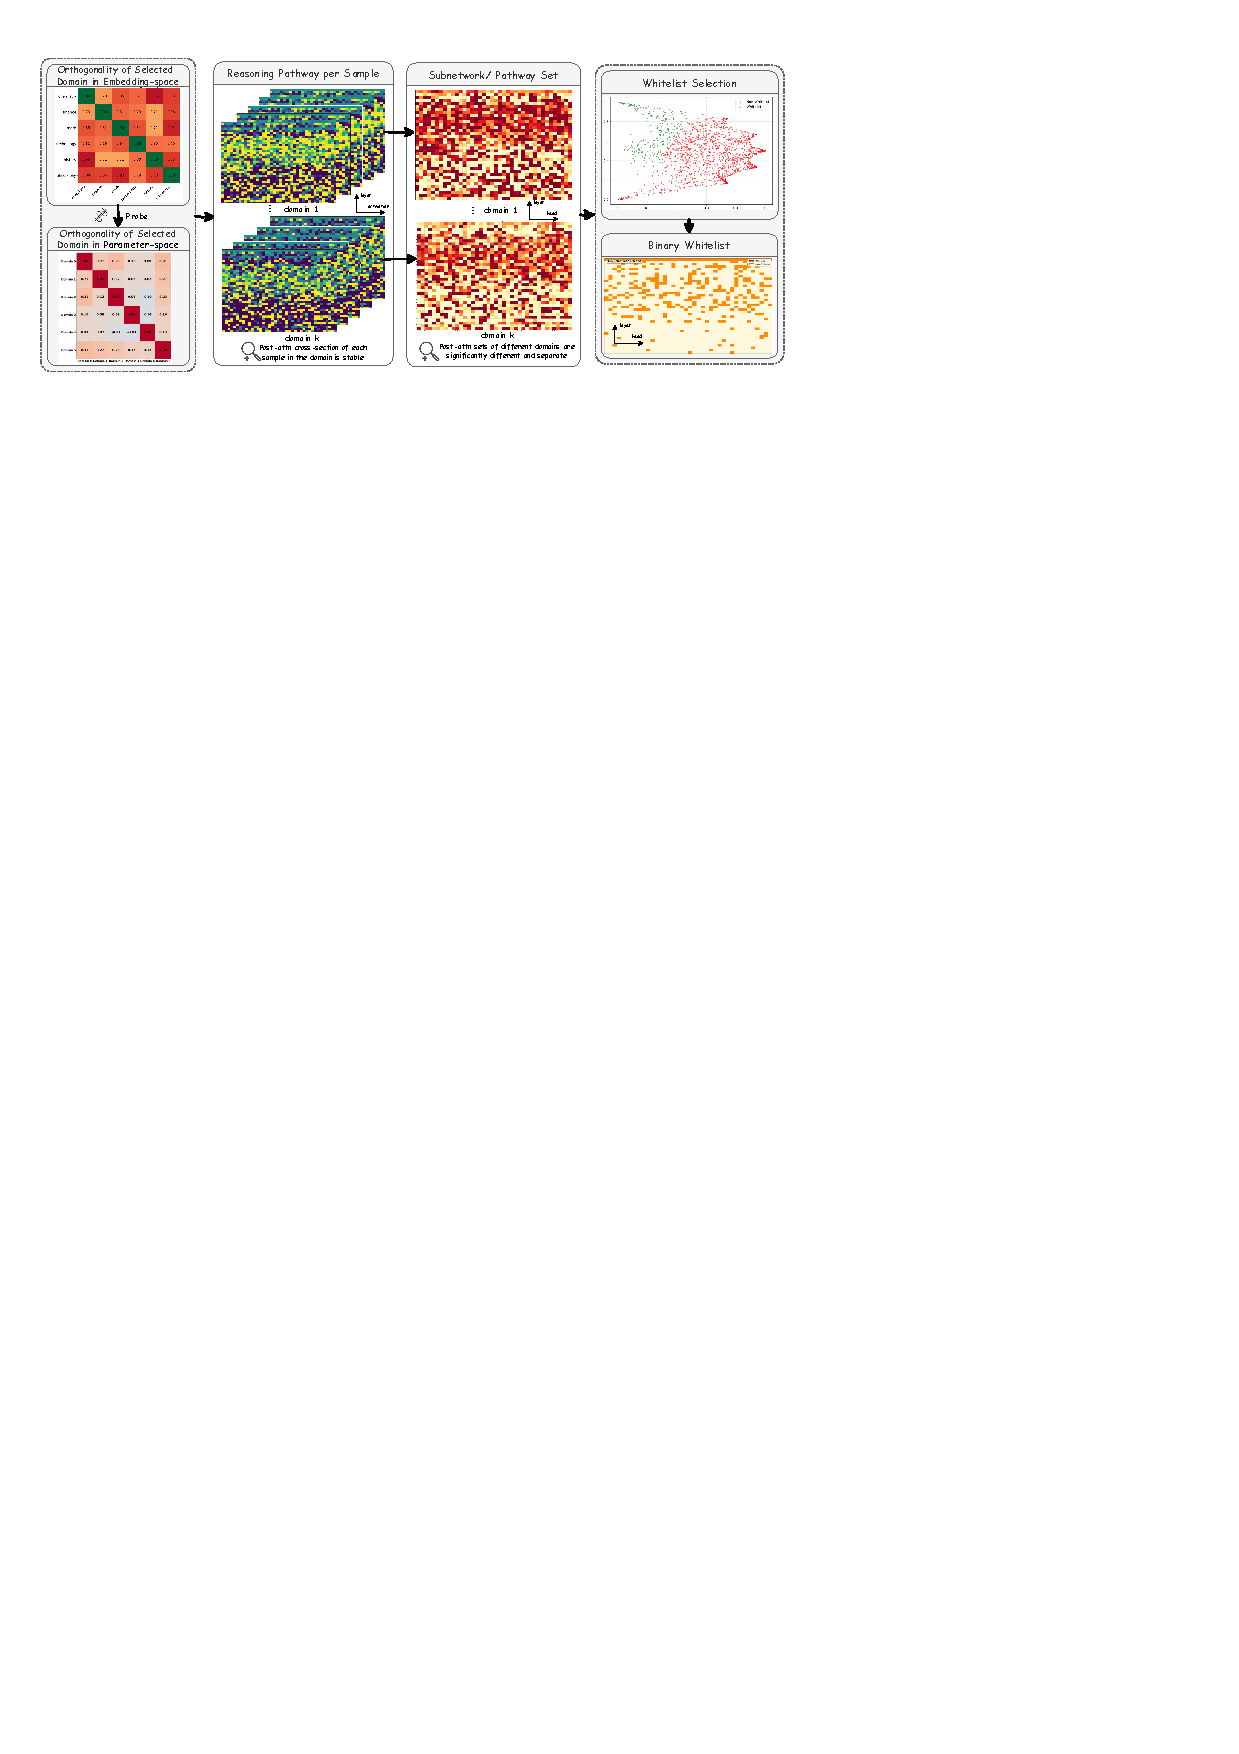
\includegraphics[width=0.95\linewidth]{figs/Subspace–pathway coupling signal1.pdf}
\vspace{-2mm}
\caption{\textbf{Subspace--pathway coupling.}
Embedding-level axes provide a stable coordinate system; probe-based axis alignment readouts from residual slices correlate with head-level pathway, enabling scenario-specific compilation of budget-bounded pathway pruning.}
\label{fig:align_pathway}
\end{figure*}

\vspace{-2pt}
\section{Methodology}
\label{sec:method}
\vspace{-2pt}
% \subsection{Overview}
% \label{sec:method_overview}
% \textbf{Overview.} We set up the empirical pipeline in \cref{sec:prelim_empirical} into a practical \emph{scenario-level compilation} mechanism based on the problem setting in \cref{sec:prelim_problem}. 
% Crucially, our \emph{inference-time stage is training-free}: there is no need to perform optimization during online inference.
% All lightweight learning happens in an offline stage using input-only pools $\{\mathcal{P}_k\}_{k\in\mathcal{K}}$.
% The \emph{offline} stage (\cref{sec:method_offline}) produces a coupled toolkit with two core components:
% \textbf{DBS} constructs a selected axis basis $\mathbb{U}_\star$ in embedding space as a stable coordinate;
% \textbf{PSP (offline)} trains layer-wise linear probes aligned to $\mathbb{U}_\star$, caches head importance statistics and whitelist.
% At the \emph{online} stage (\cref{sec:method_online}), \textbf{PSP (online)} evaluates probes on the scenario's initial inputs, combines the resulting axis alignment with cached importance to compile a pruning $m_s$ under budget $B$, and reuses $m_s$ for all subsequent turns. The complete algorithm pipeline is shown in Appendix~\ref{app:complete_pipeline}.
\textbf{Overview.} Following the principles in \cref{sec:prelim_problem,sec:prelim_empirical}, our framework operates as a training-free, scenario-level compiler that separates lightweight learning from real-time inference. Specifically, the offline stage (\cref{sec:method_offline}) utilizes input-only pools $\{\mathcal{P}_k\}$ to construct a stable coordinate basis $\mathbb{U}_\star$ via \textbf{DBS}, while \textbf{PSP} trains layer-wise probes and caches importance aligned to these axes.At online inference (\cref{sec:method_online}), \textbf{PSP} evaluates the initial scenario inputs against the pre-trained probes to resolve axis alignment. This signal is combined with cached importance to compile a pruning mask $m_s$ under budget $B$, which is then reused for all subsequent turns to ensure zero optimization overhead during deployment. The complete algorithm pipeline is shown in Appendix~\ref{app:complete_pipeline}.
\vspace{-1mm}

\subsection{Offline Preparation}
\label{sec:method_offline}
\vspace{-2pt}

\subsubsection{Domain-Basis Synthesis (DBS)}
\label{sec:method_dbc}
\vspace{-1mm}


\textbf{Stopword filtering and PCA of embedding.}
Let $\mathcal{S}$ be a fixed stopword list.
For each input sequence $x$, we remove tokens in $\mathcal{S}$ to obtain $\tilde{x}$.
We then compute an embedding $\mathbf{e}(x)=\phi(\tilde{x})\in\mathbb{R}^d$ as in \cref{sec:prelim_notation}. Token repetition is preserved in $\mathcal{\tilde{P}}_k=\{\tilde{x}_i\}_{i=1}^{N_k}$ and thus contributes to a \emph{density signature}~\cite{manning2008ir}. We construct a shared PCA projection matrix $P\in\mathbb{R}^{d\times d'}$ with $d' = M-1$ on the pooled embeddings, where $P$ stacks the top-$d'$ principal directions~\cite{jolliffe2002pca}.
We then project by $\tilde{\mathbf e}(x)=P^\top \mathbf e(x)\in\mathbb{R}^{d'}$.
Although centroid-based, each axis is built after lexical denoising and shared PCA projection and selected by orthogonality--coverage, serving as a stabilized semantic anchor rather than a naive token average.
%This choice follows a standard multi-class geometry principle: for $M$ groups, the between-group scatter (spanned by class mean differences) has rank at most $M-1$, so an $(M\!-\!1)$-dimensional subspace is sufficient to preserve all degrees of freedom for separating $M$ groups (e.g., in LDA-style analyses; \citealp{fisher1936use,fukunaga1990spr,hastie2009esl}; formal argument in \cref{app:math_pca_dim}). Additional theoretical analysis and mathematical properties are provided in \cref{app:math_configuration}.

\textbf{Domain subset selection.}
We first construct a candidate axis from each pool.
For each pool $k\in\mathcal{K}$, we compute the centroid in the PCA space~\cite{rocchio1971relevance}: $\boldsymbol{\mu}_k \;=\; \frac{1}{\left|\mathcal{P}_k\right|}\sum_{x\in\mathcal{P}_k} \tilde{\mathbf e}(x)$, $\mathbf{u}_k \;=\; \frac{\boldsymbol{\mu}_k}{\left\|\boldsymbol{\mu}_k\right\|_2}\in\mathbb{R}^{d'}$,
Here we treat the \emph{axis} as $\mathcal{U}_k=\mathrm{span}(\mathbf{u}_k)$ and denote $\mathbb{U}=\{\mathcal{U}_k\}_{k\in\mathcal{K}}$.

We then implement domain subset selection with the objective of orthogonality and coverage.
We select a compact axis set $\mathcal{K}_\star\subseteq\mathcal{K}$ by balancing:

\emph{(i) Orthogonality.} For a subset $\mathcal{K}'$, define
{\small
\begin{equation}
\label{eq:dbc:ortho}
\mathrm{Ortho}(\mathcal{K}')
\;=\;
1-\frac{2}{\lvert\mathcal{K}'\rvert(\lvert\mathcal{K}'\rvert-1)}
\sum_{i<j,\; i,j\in\mathcal{K}'}
\left(\mathbf{u}_i^\top \mathbf{u}_j\right)^2,
\end{equation}
}
which penalizes axis overlap~\cite{bjorck1973angles}.

\emph{(ii) Coverage.} Let $\Sigma$ be the global covariance of all pooled embeddings in the PCA space:
$\Sigma=\mathrm{Cov}\left(\left\{\tilde{\mathbf e}\left(x\right): x\in\cup_k\mathcal{P}_k\right\}\right)$.
Let $U(\mathcal{K}')$ be the matrix whose columns are $\{\mathbf{u}_k\}_{k\in\mathcal{K}'}$ and
$\Pi(\mathcal{K}')$ be the projection matrix onto $\mathrm{span}(U(\mathcal{K}'))$
(orthonormalization implied). Define
\begin{equation}
\label{eq:dbc:cover}
\mathrm{Cover}(\mathcal{K}')
\;=\;
\frac{\mathrm{tr}\!\left(\Pi\left(\mathcal{K}'\right)\,\Sigma\right)}{\mathrm{tr}(\Sigma)}\in[0,1],
\end{equation}
measuring how much global semantic variance is captured by the selected axes~\cite{jolliffe2002pca}. We then maximize a combined score:
\begin{equation}
\label{eq:dbc:objective}
J(\mathcal{K}') \;=\; \lambda_{\mathrm{ortho}}\cdot \mathrm{Ortho}(\mathcal{K}')
\;+\; \lambda_{\mathrm{cov}}\cdot \mathrm{Cover}(\mathcal{K}').
\end{equation}
In practice, we use greedy screening to detect the elbow point, as detailed in Appendix~\ref{app:dbc_details}.
The selected basis is $\mathbb{U}_\star=\{\mathcal{U}_k\}_{k\in\mathcal{K}_\star}$~\cite{satopaa2011finding}.

%\subsubsection{Parameter Pathway Decoupling (PPD)}
%\label{sec:method_ppd}

%DBC provides a quasi-orthogonal axis coordination, but Evidence~3 shows that pathway sets are only partially separable (\cref{sec:prelim_empirical}).
%So, we introduce PPD, an \emph{offline decoupling} step, to make axis-aligned pathway sets more separable, \emph{not} to maximize task accuracy, but to improve the reliability of the subsequent probe-based scenario pruning (PSP).

%\textbf{Decoupling on non-foundation layers.}
%We first identify foundation layers $\mathcal{L}_0\subseteq\{1,\dots,L\}$ whose domain relevance is approximately uniform across $k\in\mathcal{K}_\star$ (general-purpose layers; identified using the same probe signals in \cref{sec:method_psp_offline}).
%We then apply a lightweight LoRA parameterization only on layers $\ell\notin\mathcal{L}_0$ to obtain $\theta'=\theta+\Delta\theta(\psi)$ \cite{hu2022lora}, while preserving the always-retained whitelist $\mathcal{W}$ (\cref{sec:prelim_empirical}) as a hard constraint in the later mask compilation.

%\textbf{Axis--layer decoupling objective.}
%Let $\mathbf{u}_k$ ($k\in\mathcal{K}_\star$) be the selected axis directions in the shared PCA space (\cref{sec:method_dbc}), and let $\tilde{\mathbf r}^{(\ell)}(x)=P^\top r^{(\ell)}(x)\in\mathbb{R}^{d'}$ denote the projected post-attention residual slice (\cref{sec:prelim_notation}).
%We define the axis-alignment energy and its induced axis distribution per layer:
%\begin{equation}
%\label{eq:ppd:pi}
%\begin{aligned}
%\alpha^{(\ell)}_k(x)
%&=\frac{\left(\mathbf{u}_k^\top \tilde{\mathbf r}^{(\ell)}(x)\right)^2}{\left\|\tilde{\mathbf r}^{(\ell)}(x)\right\|_2^2+\epsilon},
%\quad\pi^{(\ell)}(x)=\mathrm{softmax}\!\big(\alpha^{(\ell)}(x)/\tau\big),\\
%\pi^{(\ell)}&=\mathbb{E}_{x\sim \mathcal{D}_{\mathrm{ppd}}}\big[\pi^{(\ell)}(x)\big],
%\quad k\in\mathcal{K}_\star,\;\ell\notin\mathcal{L}_0,
%\end{aligned}
%\end{equation}
%where $\mathcal{D}_{\mathrm{ppd}}$ is an offline question-only set, $\epsilon$ is a small constant for numerical stability, and $\tau$ is a softmax temperature. 
%$\pi^{(\ell)}(x)$ is the per-layer axis distribution for $x$ and $\pi^{(\ell)}$ is its expectation over $\mathcal{D}_{\mathrm{ppd}}$.

%We encourage (i) \emph{few axes per layer} via within-layer entropy, and (ii) \emph{few layers per axis} via entropy of the axis-specific layer profile:
%\begin{equation}
%\label{eq:ppd:entropies}
%\begin{aligned}
%\mathcal{L}_{\mathrm{intra}}
%&= \sum_{\ell\notin\mathcal{L}_0} H\!\left(\pi^{(\ell)}\right),
%\
%\mathcal{L}_{\mathrm{inter}}= \sum_{k\in\mathcal{K}_\star} H\!\left(\frac{\pi^{(\ell)}_k}{\sum_{j\notin\mathcal{L}_0}\pi^{(j)}_k}\right).
%\end{aligned}
%\end{equation}
%with $H(\cdot)$ the Shannon entropy \cite{shannon1948mathematical}.

%Finally, to avoid degenerate drift during decoupling,
%we add a soft prediction-consistency regularizer between the frozen base and the decoupled model
%on the same question-only inputs:
%\begin{equation}
%\label{eq:ppd:consistency}
%\mathcal{L}_{\mathrm{cons}}
%=
%\mathbb{E}_{x\sim \mathcal{D}_{\mathrm{ppd}}}
%\Big[
%\mathrm{KL}\big(p_\theta(\cdot\mid x)\,\|\,p_{\theta'}(\cdot\mid x)\big)
%\Big],
%\end{equation}
%a standard teacher--student style stabilization without labels \cite{hinton2015distilling}.
%We obtain $\psi$ by minimizing the decoupling objective
%\begin{equation}
%\label{eq:ppd:total}
%\min_{\psi}\;\mathcal{L}_{\mathrm{ppd}}
%=
%\mathcal{L}_{\mathrm{intra}}
%+
%\lambda_{\mathrm{inter}}\mathcal{L}_{\mathrm{inter}}
%+
%\lambda_{\mathrm{cons}}\mathcal{L}_{\mathrm{cons}},
%\end{equation}
%with $(\tau,\lambda_{\mathrm{inter}},\lambda_{\mathrm{cons}})$ as hyperparameters in \cref{app:ppd_details}.

\subsubsection{Probe-based scenario-level Pruning (PSP)}
\label{sec:method_psp_offline}
\vspace{-1mm}

\textbf{Layer-wise probes.}
For each layer $\ell$ and each selected domain $k\in\mathcal{K}_\star$,
we train a linear probe on the post-attention residual slice $r^{(\ell)}(\tilde{x})\in\mathbb{R}^d$.
Let $\mathbf{g}_{\ell,k}\in\mathbb{R}^d$ denote the probe weight vector (bias omitted for simplicity) and
$z_{\ell,k}(x)=\mathbf{g}_{\ell,k}^\top r^{(\ell)}(\tilde{x})$ be the probe logit.
We output a 1-vs-rest probability: \(p_{\ell,k}(x) = \sigma(z_{\ell,k}(x)) \in (0,1)\), where $\sigma$ is sigmoid~\cite{alain2016linearprobes,belinkov2022probing}.
Training uses labels over the union set $\cup_{k\in\mathcal{K}_\star}\mathcal{P}_k^{\mathrm{tr}}$:
each example from $\mathcal{P}_k^{\mathrm{tr}}$ is treated as positive for $k$ and negative for
$k'\neq k$ (independent 1-vs-rest logistic regressors).

The training objective is the binary cross-entropy loss
\begin{equation}
\label{eq:loss}
\begin{aligned}
\mathcal{L}_{\ell,k}
= &-\mathbb{E}_{x\sim \cup_{j\in\mathcal{K}_\star}\mathcal{P}_j^{\mathrm{tr}}}
\left[
y_k(x)\log p_{\ell,k}\left(x\right) \right.
\\
&\left.+ \left(1-y_k\left(x\right)\right)\log\left(1-p_{\ell,k}\left(x\right)\right)
\right],
\end{aligned}
\end{equation}
where $y_k(x)=1$ iff $x\in\mathcal{P}_k^{\mathrm{tr}}$, and $0$ otherwise.
During training, this corresponds to a standard 1-vs-rest setup with one domain label per sample.
During inference, we interpret $\{p_{\ell,k}(x)\}_{k\in\mathcal{K}_\star}$ as independent relevance scores rather than a simplex distribution, since real inputs can mix multiple knowledge axes and improve generalization.


\textbf{Head-wise importance.}
We define a head's contribution to the post-attn residual write.
Let $w_{\ell,h}(x)\in\mathbb{R}^d$ denote the residual write-back vector attributable to head
$(\ell,h)$ for input $x$ (i.e., the head-wise component added into the residual stream at layer $\ell$; \citealp{elhage2021framework}).
We compute $w_{\ell,h}(x)$ as follows.

Let $r^{(\ell)}(x)$ denote the full post-attention residual at layer $\ell$, obtained by applying the output projection $\text{o\_proj}$ to the concatenated outputs of all heads.
Let $r^{(\ell)}_{-h}(x)$ denote the residual obtained by applying $\text{o\_proj}$ to the concatenated outputs of all heads except head $h$.
Then $w_{\ell,h}(x) = r^{(\ell)}(x) - r^{(\ell)}_{-h}(x)$ to ensure that the sum of all head contributions equals the full residual and avoids bias-related artifacts from the output projection.
We map this write into the shared PCA space:
$\tilde{w}_{\ell,h}(x)=P^\top w_{\ell,h}(x)\in\mathbb{R}^{d'}$.
Then the domain-specific head importance is defined as the expected axis-aligned energy:
{\small
\begin{equation}
\label{eq:psp:importance}
\begin{aligned}
I_{\ell,h,k}
\;=\;
\mathbb{E}_{x\sim \mathcal{P}_k^{\mathrm{tr}}}
\left[
\frac{\left(\mathbf{u}_k^\top \tilde{w}_{\ell,h}\left(x\right)\right)^2}
{\left\|\tilde{w}_{\ell,h}(x)\right\|_2^2+\epsilon}
\right],
\quad k\in\mathcal{K}_\star.
\end{aligned}
\end{equation}
}
where $\epsilon$ is a small constant for numerical stability. Intuitively, $I_{\ell,h,k}$ is large if head $(\ell,h)$ consistently writes along the selected
embedding-axis $\mathbf{u}_k$ on domain-$k$ inputs, and small if it is irrelevant. We compute $\{I_{\ell,h,k}\}$ once offline and cache them for inference-time compilation.


\textbf{Whitelisting.}
We identify a set of always-retained heads $\mathcal{W}\subseteq \mathcal{H}$ to preserve general-purpose capacity.
We select a set of domain-invariant \emph{backbone heads} by statistical significance testing.
Specifically, for each head $(\ell,h)$, we compute its importance variance across domains:
$\sigma_{\ell,h} = \mathrm{Std}(\{I_{\ell,h,k}: k\in\mathcal{K}_\star\})$ and mean importance:
$\mu_{\ell,h} = \frac{1}{|\mathcal{K}_\star|}\sum_{k\in\mathcal{K}_\star} I_{\ell,h,k}$.
We retain heads that exhibit low domain variance (indicating domain-invariance) and sufficient average importance:
{\small
\begin{equation}
\label{eq:psp:whitelist_backbone}
\mathcal{W}_{\mathrm{bb}}
\;=\;
\left\{
\left(\ell,h\right)\in\mathcal{H}:\;
\sigma_{\ell,h} \leq \sigma_{\mathrm{thresh}},\;
\mu_{\ell,h} \geq \mu_{\mathrm{thresh}}
\right\},
\end{equation}
}
where $\sigma_{\mathrm{thresh}}$ and $\mu_{\mathrm{thresh}}$ are thresholds determined by statistical significance testing.
Keep $\mathcal{W}=\mathcal{W}_{\mathrm{bb}}$ always during compilation.
Statistical validation confirms that whitelisted heads have significantly lower domain variance than non-whitelisted heads (Mann-Whitney U test, $p<0.001$; Algorithm details in Appendix ~\ref{app:whitelist_details}).

\definecolor{icmlblue}{RGB}{235, 243, 255} 
\definecolor{lightgray}{gray}{0.96}        

\begin{table*}[t]
\caption{\textbf{Performance comparison of \textsc{SubspacePath Pruner} at different pruning ratios for LLaMA-2-13B-chat across various datasets.}
Token-level Recall (Recall) values shown as mean ±  standard error of the mean (SEM). Retention = $(\text{Recall}_{\text{pruned}} / \text{Recall}_{\text{dense}}) \times \text{Speedup}$.
Pruning ratios: left value (baseline), right value (ours, average); ours prunes more aggressively.}
\vspace{-2mm}
\centering
\footnotesize 
\setlength{\tabcolsep}{2.8pt} 
\renewcommand{\arraystretch}{1.02} % 1. 显著收紧行高倍数
\resizebox{0.98\textwidth}{!}{%
\begin{tabular}{p{1.1cm}p{1.2cm} c c c c c c c c c c c c c c c c c c c c c c c c c c c c c c c c c c c c c c c c c c c c c c c c c c c c c c c c c c c c c c c c c c c c c c c c c c c c c c c c c c c c c c c c c c c c c c c c c c c c c c} 
\toprule
% 2. 使用更紧凑的表头结构
\textbf{Category} & \textbf{Method} & \multicolumn{3}{c}{\textbf{XdomainBench}} & \textbf{Retention} & \multicolumn{3}{c}{\textbf{Cross-dataset Test}} & \textbf{Retention} \\ 
\cmidrule(r){3-5} \cmidrule(lr){6-6} \cmidrule(lr){7-9} \cmidrule(l){10-10}
 &  & \textbf{Selected} & \textbf{OOD} & \textbf{Cross} & \textbf{(S/O/C)} & \textbf{CSQA} & \textbf{NQ} & \textbf{ARC} & \textbf{(C/N/A)} \\ 
\midrule

% Dense Model
\rowcolor{lightgray} \multicolumn{10}{c}{\rule{0pt}{1.8ex}\textbf{Dense Model}\rule[-0.6ex]{0pt}{0pt}} \\
\multicolumn{2}{l}{LLaMA-2-13B} & 29.6{\scriptsize$\pm$1.45} & 26.1{\scriptsize$\pm$1.10} & 18.4{\scriptsize$\pm$0.74} & 1.00 / 1.00 / 1.00 & 22.27{\scriptsize$\pm$1.20} & 30.25{\scriptsize$\pm$1.07} & 23.87{\scriptsize$\pm$0.89} & 1.00 / 1.00 / 1.00 \\
\midrule

% Moderate Pruning
\rowcolor{lightgray} \multicolumn{10}{c}{\rule{0pt}{1.8ex}\textbf{Moderate Pruning Ratio}\rule[-0.6ex]{0pt}{0pt}} \\ 
\rowcolor{lightgray} &  & 80\%{\scriptsize$\sim$79.6\%} & 89\%{\scriptsize$\sim$88.4\%} & 86\%{\scriptsize$\sim$85.5\%} &  & 90\%{\scriptsize$\sim$89.9\%} & 82\%{\scriptsize$\sim$81.5\%} & 81\%{\scriptsize$\sim$80.2\%} &  \\ 
\cmidrule(r){3-3} \cmidrule(lr){4-4} \cmidrule(lr){5-5} \cmidrule(lr){6-6} \cmidrule(lr){7-7} \cmidrule(lr){8-8} \cmidrule(lr){9-9} \cmidrule(l){10-10}
\multirow{2}{*}{Unstruct.} & 
% SparseGPT & 29.10{\scriptsize$\pm$}xx & 28.34{\scriptsize$\pm$}xx & 20.32{\scriptsize$\pm$}xx & 0.98 / 1.08 / 1.10 & 21.87{\scriptsize$\pm$}xx & 28.37{\scriptsize$\pm$}xx & 23.98{\scriptsize$\pm$}xx & 0.98 / 0.93 / 1.00 \\
 % & 
 DaSS & 33.82{\scriptsize$\pm$1.56} & 28.62{\scriptsize$\pm$1.16} & 19.89{\scriptsize$\pm$0.79} & 0.42 / 0.49 / 0.50 & \textbf{20.10}{\scriptsize$\pm$1.14} & 18.80{\scriptsize$\pm$0.96} & 19.22{\scriptsize$\pm$0.82} & 0.24 / 0.15 / 0.35 \\
\multirow{3}{*}{Struct.} & Wanda & 26.87{\scriptsize$\pm$1.46} & 27.26{\scriptsize$\pm$1.14} & 15.43{\scriptsize$\pm$0.74} & 0.35 / 0.46 / 0.45 & 17.63{\scriptsize$\pm$1.09} & 17.27{\scriptsize$\pm$0.98} & 14.38{\scriptsize$\pm$0.75} & 0.18 / 0.11 / 0.24 \\
     & LLM-Pr. & 29.34{\scriptsize$\pm$1.49} & 27.81{\scriptsize$\pm$1.14} & 18.92{\scriptsize$\pm$0.75} & 0.95 / \underline{1.02} / 0.99 & \textbf{21.08}{\scriptsize$\pm$1.17} & 27.63{\scriptsize$\pm$1.14} & \textbf{23.09}{\scriptsize$\pm$0.89} & 0.91 / 0.88 / 0.94 \\
 % & FASP & XX{\scriptsize$\pm$}xx & XX{\scriptsize$\pm$}xx & XX{\scriptsize$\pm$}xx & --- / --- / --- & XX{\scriptsize$\pm$}xx & XX{\scriptsize$\pm$}xx & XX{\scriptsize$\pm$}xx & --- / --- / --- \\
\multirow{2}{*}{Activ.} & RIA & 27.06{\scriptsize$\pm$1.47} & 27.03{\scriptsize$\pm$1.14} & 15.12{\scriptsize$\pm$0.73} & 0.36 / 0.47 / 0.46 & 17.98{\scriptsize$\pm$1.10} & 17.24{\scriptsize$\pm$0.98} & 14.33{\scriptsize$\pm$0.75} & 0.19 / 0.12 / 0.25 \\
 & Probe Pr. & 29.02{\scriptsize$\pm$1.58} & 27.81{\scriptsize$\pm$1.28} & 19.08{\scriptsize$\pm$1.12} & \underline{1.22} /\underline{1.33} / \underline{1.24} & \textbf{21.75}{\scriptsize$\pm$1.30} & 27.64{\scriptsize$\pm$1.41} & \textbf{23.32}{\scriptsize$\pm$1.34} & \underline{1.17} / \underline{1.09} / \underline{1.17} \\
\rowcolor{icmlblue} \multicolumn{2}{l}{\textbf{Ours-SubspacePath}} & \textbf{43.00{\scriptsize$\pm$2.40}} & \textbf{32.50{\scriptsize$\pm$1.90}} & \textbf{20.20{\scriptsize$\pm$3.00}} & \underline{1.48} / \underline{1.56} / \underline{1.78} & \textbf{19.43{\scriptsize$\pm$1.14}} & \textbf{33.66{\scriptsize$\pm$1.35}} & \textbf{22.91{\scriptsize$\pm$1.08}} & 0.94 / \underline{1.20} / \underline{2.12} \\
\midrule

% Aggressive Pruning
\rowcolor{lightgray} \multicolumn{10}{c}{\rule{0pt}{1.8ex}\textbf{Aggressive Pruning Ratio}\rule[-0.6ex]{0pt}{0pt}} \\
\rowcolor{lightgray} &  & 71\%{\scriptsize$\sim$71.0\%} & 83\%{\scriptsize$\sim$82.8\%} & 72\%{\scriptsize$\sim$71.3\%} &  & 82\%{\scriptsize$\sim$81.2\%} & 70\%{\scriptsize$\sim$69.5\%} & 69\%{\scriptsize$\sim$68.3\%} &  \\ 
\cmidrule(r){3-3} \cmidrule(lr){4-4} \cmidrule(lr){5-5} \cmidrule(lr){6-6} \cmidrule(lr){7-7} \cmidrule(lr){8-8} \cmidrule(lr){9-9} \cmidrule(l){10-10}
\multirow{2}{*}{Unstruct.} & 
% SparseGPT & 27.61{\scriptsize$\pm$}xx & 27.00{\scriptsize$\pm$}xx & 19.52{\scriptsize$\pm$}xx & 0.93 / 1.03 / 1.06 & 21.55{\scriptsize$\pm$}xx & 26.92{\scriptsize$\pm$}xx & 23.39{\scriptsize$\pm$}xx & 0.96 / 0.89 / 0.98 \\
 % & 
 DaSS & \textbf{35.27}{\scriptsize$\pm$1.57} & 27.84{\scriptsize$\pm$1.15} & 15.40{\scriptsize$\pm$0.71} & 0.87 / 0.84 / 0.80 & 18.13{\scriptsize$\pm$}1.10 & 12.42{\scriptsize$\pm$0.75} & 16.29{\scriptsize$\pm$0.79} & 0.49 / 0.22 / 0.72 \\
\multirow{3}{*}{Struct.} & Wanda & 18.12{\scriptsize$\pm$1.26} & 26.57{\scriptsize$\pm$1.15} & 8.77{\scriptsize$\pm$0.54} & 0.16 / 0.47 / 0.24 & 13,70{\scriptsize$\pm$0.99} & 8.09{\scriptsize$\pm$0.71} & 9.50{\scriptsize$\pm$0.64} & 0.17 / 0.06/ 0.31 \\
 & LLM-Pr. & 27.30{\scriptsize$\pm$1.46} & 28.15{\scriptsize$\pm$1.15} & 17.36{\scriptsize$\pm$0.71} & 0.60 / \underline{1.05} / 0.61 & \textbf{21.20}{\scriptsize$\pm$1.18} & 19.12{\scriptsize$\pm$0.95} & 21.01{\scriptsize$\pm$0.82} & 0.92 / 0.49 / 0.70 \\
 % & FASP & XX{\scriptsize$\pm$}xx & XX{\scriptsize$\pm$}xx & XX{\scriptsize$\pm$}xx & --- / --- / --- & XX{\scriptsize$\pm$}xx & XX{\scriptsize$\pm$}xx & XX{\scriptsize$\pm$}xx & --- / --- / --- \\
\multirow{2}{*}{Activ.} & RIA & 18.94{\scriptsize$\pm$1.28} & 26.69{\scriptsize$\pm$1.15} & 8.52{\scriptsize$\pm$0.54} & 0.33 / 0.91 / 0.45 & 12.48{\scriptsize$\pm$0.93} & 8.06{\scriptsize$\pm$0.71} & 9.75{\scriptsize$\pm$0.64} & 0.31 / 0.10 / 0.32 \\
 & Probe Pr. & 15.19{\scriptsize$\pm$1.25} & 27.84{\scriptsize$\pm$1.28} & 11.54{\scriptsize$\pm$0.91} & 0.43 / \underline{1.29} / 0.52 & \textbf{21.65}{\scriptsize$\pm$1.30} & 11.34{\scriptsize$\pm$1.00} & 6.96{\scriptsize$\pm$0.80} & \underline{1.19} / 0.31 / 0.25 \\
\rowcolor{icmlblue} \multicolumn{2}{l}{\textbf{Ours-SubspacePath}} & \textbf{34.70{\scriptsize$\pm$2.30}} & \textbf{30.40{\scriptsize$\pm$1.90}} & \textbf{22.90{\scriptsize$\pm$3.20}} & \underline{1.24} / \underline{1.36} / \underline{1.92} & \textbf{18.40{\scriptsize$\pm$1.12}} & \textbf{24.89{\scriptsize$\pm$1.22}} & \textbf{21.56{\scriptsize$\pm$1.04}} & 0.65 / 0.80 / \underline{1.59} \\
\bottomrule
\end{tabular}}
\vspace{-1mm}
\label{tab:psp_results}
\end{table*}

\begin{table}[t]
\centering
\caption{\textbf{Pruning Time \& Speedup} on RTX A6000. Speedup is reported as light/aggressive. The complete results are in Table~\ref{tab:pruning_time}.}
\vspace{-2mm}
\footnotesize
\setlength{\tabcolsep}{2.2pt}   % tighter to avoid overflow
\renewcommand{\arraystretch}{1.05}
\resizebox{\linewidth}{!}{%
\begin{tabular}{l c c c c}
\toprule
\textbf{Pruning Time (s) $\downarrow$} & \scriptsize\textbf{LLaMA-8B} & \scriptsize\textbf{LLaMA-13B} & \scriptsize\textbf{Qwen-7B} & \scriptsize\textbf{Qwen-14B} \\
\midrule
Wanda & 0.137 & 0.525 & 0.098 & 0.558 \\
LLM-Pr & 0.340 & 0.593 & 0.266 & 0.599 \\
RIA & 0.083 & 0.275 & 0.078 & 0.290 \\
\rowcolor{icmlblue} \textbf{Ours-SubspacePath} & \textbf{0.039} & \textbf{0.060} & \textbf{0.027} & \textbf{0.068} \\
\midrule
\textbf{Speedup $\uparrow$} & \scriptsize\textbf{LLaMA-8B} & \scriptsize\textbf{LLaMA-13B} & \scriptsize\textbf{Qwen-7B} & \scriptsize\textbf{Qwen-14B} \\
\midrule
Wanda & 0.48 / 0.19 & 0.39 / 0.42 & 0.22 / 0.13 & 0.28 / 0.32 \\
LLM-Pr & 0.61 / 0.64 & 0.96 / 0.80 & 0.66 / 0.67 & 0.96 / 0.66 \\
RIA & 0.36 / 0.19 & 0.40 / 0.74 & 0.29 / 0.13 & 0.29 / 0.32 \\
\rowcolor{icmlblue} \textbf{Ours-SubspacePath} & \textbf{1.41/1.35} & \textbf{3.22/1.51} & \textbf{2.01/0.88} & \textbf{1.38/1.29} \\
\bottomrule
\end{tabular}%
}
\vspace{-1mm}
\label{tab:pruning_time_main}
\end{table}
  
\subsection{Online Probe-based Scenario-level Pruning}
\label{sec:method_online}
\vspace{-1mm}

Given a new scenario $s$, we compile a reusable pruning $m_s$ under a budget $B$ using only the
first $T_0$ inputs.
In practice, we compile the mask from the first scenario input only, relying on the shared semantic signal of a coherent scenario rather than future-turn information.
All probe evaluations are performed on the frozen backbone $f_{\theta}$.

\textbf{Scenario-level domain mixture and head scoring.}
For each layer $\ell$ and domain $k$, we aggregate the probe outputs over stopword-filtered input $\tilde{x}_t$: \(\bar p_{\ell,k}(s) = \frac{1}{T_0}\sum_{t=1}^{T_0} \hat p_{\ell,k}(\tilde{x}_t)\).
We further define a scenario-level domain mixture by pooling over layers: \(q_k(s) = \frac{1}{L}\sum_{\ell=1}^{L}\bar p_{\ell,k}(s)\), \(k\in\mathcal{K}_\star\).
We then quantify scenario knowledge breadth using the normalized entropy:
{\small
\begin{equation}
\label{eq:on:breadth}
\begin{aligned}
H(q(s))
&= -\sum_{k\in\mathcal{K}_\star}
\frac{q_k(s)}{\sum_{j\in\mathcal{K}_\star} q_j(s)}
\log\!\left(\frac{q_k(s)}{\sum_{j\in\mathcal{K}_\star} q_j(s)}\right),\\
c(s)
&= \frac{H\left(q\left(s\right)\right)}{\log |\mathcal{K}_\star|}\in[0,1].
\end{aligned}
\end{equation}
}
Low $c(s)$ indicates a narrow scenario; high $c(s)$ indicates a broader cross-domain scenario.
We score heads based on alignment and cached importance.
For each domain $k$, we compute domain-specific head scores using an effective domain similarity $s_k^{\text{eff}}$ that is obtained via a non-linear transformation of the raw domain similarity $q_k(s)$ (\cref{eq:domain_keep_ratio_improved}).
The effective similarity amplifies high similarities to preserve more heads for highly relevant domains while reducing preservation for less relevant domains.
The final head score aggregates across all domains:
{\small
\begin{equation}
\vspace{-5pt}
\label{eq:on:score}
\mathrm{score}_{\ell,h}(s)
\;=\;
\sum_{k\in\mathcal{K}_\star} s_k^{\text{eff}} \cdot I_{\ell,h,k},
\vspace{-5pt}
\end{equation}
}
where $s_k^{\text{eff}}$ is the effective domain similarity for domain $k$ after non-linear transformation.
This instantiates the subspace--pathway coupling: probe alignment indicates \emph{what the scenario needs}, and $I_{\ell,h,k}$ indicates \emph{which heads realize that axis}.
The non-linear transformation ensures more precise pruning by avoiding under-pruning highly relevant domains while reducing over-preservation of less relevant domains.


\textbf{Budget, pruning strength, and pruning compilation.}
We treat the inference budget $B$ as a constraint on the pruned model cost $\mathcal{C}\left(f_{\theta'}^{\left(m_s\right)}\right) \le B$.
Since exact cost is hardware-dependent, we implement the budget via an equivalent head budget $K_B$ (e.g., a mapping from heads to latency/memory).
We introduce a single \emph{pruning-strength} hyperparameter $\eta \in (0, 1]$ that controls the overall aggressiveness, and let the scenario breadth $c(s)$ modulate the effective keep-ratio:
%\vspace{-0.5mm}
{\small
\begin{equation}
\label{eq:on:Ks}
\begin{split}
K(s)
&= |\mathcal{W}|
 + \min\Big\{
   K_B-|\mathcal{W}|,\,
\\
&\qquad\qquad
   \Big\lceil\big(\rho_{\min}+\eta\,c(s)\big)\big(|\mathcal{H}|-|\mathcal{W}|\big)\Big\rceil
 \Big\}.
\end{split}
\end{equation}
}
\vspace{-0.5mm}
where $\rho_{\min}$ is a fixed small floor keep-ratio.
Thus, small $c(s)$ in narrow scenarios, fewer heads are kept; broad scenarios kept more, while $\eta$ globally scales pruning strength. After determining the keep budget, we always retain whitelist $\mathcal{W}$ and select remaining $K(s) - |\mathcal{W}|$ heads with the largest $\mathrm{score}_{\ell,h}(s)$ (ties broken deterministically), producing a binary sign $m_s \in \{0, 1\}^{|\mathcal{H}|}$ and an executable pruned instance $f_{\theta}^{(m_s)}$. Algorithm details are in Appendix ~\ref{app:budget_mapping}.
\vspace{-0.5mm}
%In the main experiments, we choose $\eta$ at an empirical elbow point: increasing $\eta$ beyond it yields diminishing performance gains but significantly more parameters, while decreasing $\eta$ below it starts to reduce performance (trade-off quantified in \cref{app:eta_tradeoff}).